\documentclass[12pt]{article}
\usepackage{geometry} 
\geometry{a4paper}
\usepackage{listings}
\usepackage[utf8]{inputenc}
\usepackage{listings}
\usepackage{xcolor}
\usepackage{graphicx}
\usepackage{float}
\usepackage{caption}
\usepackage{subcaption}
\usepackage{amsmath}
\usepackage{algorithm}
\usepackage[noend]{algpseudocode}
\usepackage[shortlabels]{enumitem}
\usepackage[overload]{empheq}

\definecolor{codegreen}{rgb}{0,0.6,0}
\definecolor{codegray}{rgb}{0.5,0.5,0.5}
\definecolor{codepurple}{rgb}{0.58,0,0.82}
\definecolor{backcolour}{rgb}{0.95,0.95,0.92}
\lstdefinestyle{mystyle}{
	backgroundcolor=\color{backcolour},   
	commentstyle=\color{codegreen},
	keywordstyle=\color{magenta},
	numberstyle=\tiny\color{codegray},
	stringstyle=\color{codepurple},
	basicstyle=\ttfamily\footnotesize,
	breakatwhitespace=false,         
	breaklines=true,                 
	captionpos=b,                    
	keepspaces=true,                 
	numbers=left,                    
	numbersep=5pt,                  
	showspaces=false,                
	showstringspaces=false,
	showtabs=false,                  
	tabsize=2
}
\lstset{style=mystyle}

\title{Assignment 5}
\author{Umberto Cocca}
\date{} 

\begin{document}
\maketitle
\noindent \textbf{Problem 1}\\

\begin{itemize}
	\item First of all we compute the number of the triangles in a triangulation considering that each edge bounds two triangles if they aren't convex hull edges, otherwise the edge bounds one triangle. Since a triangle has 3 edges we state:
	\begin{equation}
		\begin{aligned}
			3t &= 2(E-h)+h \\
			&= 2E -h
		\end{aligned}
	\end{equation}
	So we have a formula for $E$ and $t$:
	\begin{equation} \label{eq:1}
		\begin{aligned} 
			E &= \dfrac{3t+h}{2} \\
		\end{aligned}
	\end{equation}
	\begin{equation} \label{eq:2}
		\begin{aligned} 
			t &= \dfrac{2E-h}{3} \\
		\end{aligned}
	\end{equation}
	
	Euler's formula:
	\begin{equation} 
		\begin{aligned} 
			V - E + F &= 2 \\
		\end{aligned}
	\end{equation}
	
	Since the number of vertices is $n$ and the number of facets are $t+1$:
	\begin{equation} \label{eq:3}
		\begin{aligned}
			n-E+t &= 1 \\
		\end{aligned}
	\end{equation}
	
	Now, if we substituite (\ref{eq:1}) and (\ref{eq:2}) in (\ref{eq:3}) we obtain respectively:
	\begin{equation}
		\begin{aligned}
			t &= 2n - h - 2 \\
		\end{aligned}
	\end{equation}
	
	\begin{equation}
		\begin{aligned}
			E &= 3n - h - 3 \\
		\end{aligned}
	\end{equation}
	
	Therefore, all convex hull vertices are all the vertices ($h=n$) we obtain that the number of triangles is:
	\begin{equation}
		\begin{aligned}
			t &= 2n - n - 2 \\
			&= n-2
		\end{aligned}
	\end{equation}
	
	and the number of edges (including the edges of the convex hull) is:
	\begin{equation}
		\begin{aligned} \label{eq:4}
			E &= 3n - n - 3 \\
			&= 2n - 3
		\end{aligned}
	\end{equation}
	
	\item If we add up the degree of all vertices in a graph (in any graph) this is equal to $E$. Even if it's not a planar graph. For a planar graph we know that:
	\begin{equation}
		\begin{aligned}
			E & \leq 3(V-2) \\
		\end{aligned}
	\end{equation}
	
	For the delaunay triangulation we know a little more:
	\begin{equation}
		\begin{aligned}
			E &= 3n - 3 - h \\
		\end{aligned}
	\end{equation}
	
	where $n$ are the number of vertices not on the convex hull, hence $E < 3n$ and we can state:
	\begin{equation}
		\begin{aligned}
			\sum d(v) &= 2E < 6n \\
			\dfrac{ \sum d(v) } {n} &< \dfrac{6n}{n} = 6
		\end{aligned}
	\end{equation}
	
	This mean that in the delaunay triangulation the average vertex degree is strictly $< 6$.
	
	For the specific problem we know $E = 2n - 3$ from (\ref{eq:4}), hence $E < 2n$ and we can state:
	\begin{equation}
		\begin{aligned}
			\sum d(v) &= 2E < 4n \\
			\dfrac{ \sum d(v) } {n} &< \dfrac{4n}{n} = 4
		\end{aligned}
	\end{equation}
	
	\item The number of structural changes is equal to $p$'s degree after insertion. Let $d_i$ be a random variable that indicates the degree of the newly inserted site. Let $P_i = {p_1, ... p_i}$ denote the first $i$ sites to be inserted where $4 \leq i \leq n$. Because the diagram doesn't depend on the insertion order, each of the sites of $P_i$ has an equal prob of $\dfrac{1}{i}$ of being the last site inserted:
	\begin{equation}
		\begin{aligned}
			E_i &= 3n - 3 - h \\
		\end{aligned}
	\end{equation}
	
	Since $n,h=i$
	\begin{equation}
		\begin{aligned}
			E_i &= 2i - 3 \\
			E_i &< 2i
		\end{aligned}
	\end{equation}
	
	Now we can compute the expected number of structural changes following the insertion of the $i$th site:
	\begin{equation}
		\begin{aligned}
			E[d_i] &= \dfrac{1}{i} \sum_{j=1}^{i} deg(p_i) \\
			&= \dfrac{1}{i} 2 E_i < \dfrac{1}{i} 4i = 4
		\end{aligned}
	\end{equation}
	
\end{itemize}

\noindent \textbf{Problem 2}\\
We set $y^{-} = 0$ and $y^{+}=12$. We create a set $Sx$ that is the sort of every point of $p \in P$ resepect the $x$ coordinate. Likewise, we compute $Sy$ that is the sort of every point of $p \in P$ respect the $y$ coordinate. Sopposing $n > 1$ and point distributed not abnormally, we start identifying the distances for each point $p$ as shown in the picture below. 

\begin{figure}[H]
	\centering
	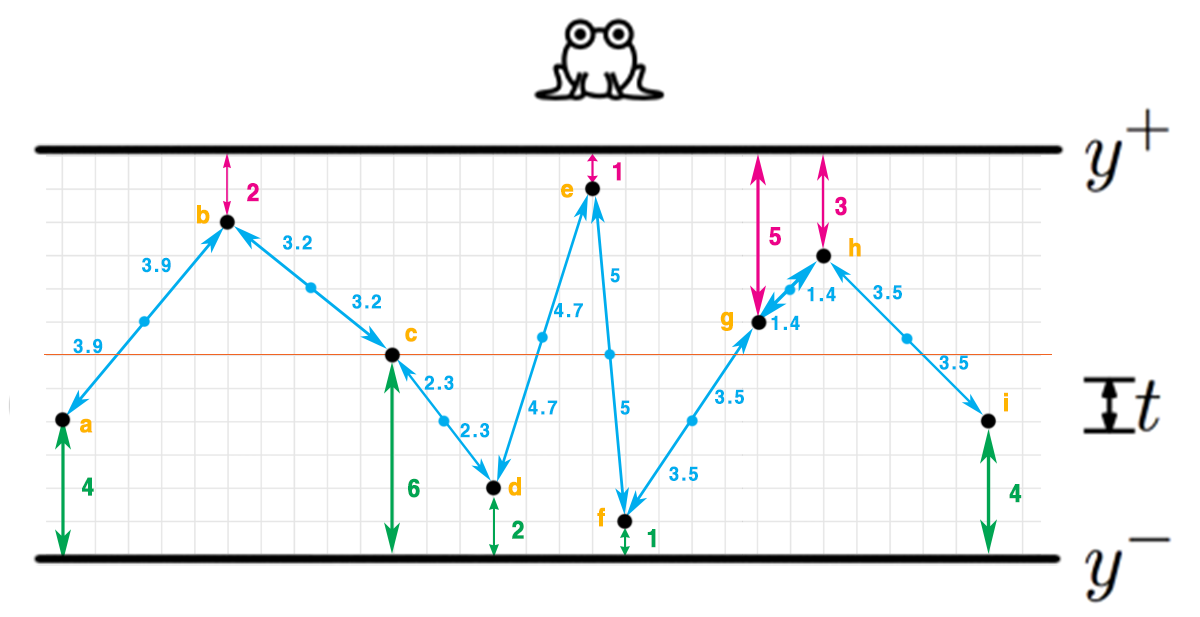
\includegraphics[scale=0.35]{img/problem2-1.png}
	\caption{For each point $p$ we compute the distances between their neighbors and their distances with $y^+$ or $y^-$ depending on their  coordinate if it is below or upper the middle between $y^+$ and $y^-$.} \label{fig:1a}
\end{figure}

\begin{lstlisting}
FrogTime():
	# here is the main
	distances = []
	
	# computing the distances as described in Figure 1
	for index, p in P:
		if p.y <= y^+ /2:
			distances.append(p.y)
		else
			distances.append(y^+ - p.y)
	
		# the first point is the most left point
		# so he has only a right neighboring 
		if p == P[0]:
			distances.append( |p - P[1]| / 2)
			
		# the last point is the most right point
		# so we compute the distance with the second last point
		if p != P[-1]:
			distances.append( |p - P[index + 1]| / 2)
	
	sort(distances) # ascending order, from min to max
	
	for t in distances:
		# plane sweep algorithm to compute the intersections
		planeSweep(t)
		
		# verify if it exists a path from y^+ to y^-
		if verify():
			return t


verify():
	for p in P:
		if p.existIntersection(y^+) and  p.existIntersection(y^-):
			return True
		
		# starting from y^+, find y^-
		if p.existIntersection(y^+):
			return findLower(p)
			
		# starting from y^-, find y^+
		if p.existIntersection(y^-):
			return findUpper(p)

# this array improves the computation while searching
alreadySeen = []

findLower(p):
	alreadySeen.append(p)
	for s in (p.intersections() not in alreadySeen):
		if s.existIntersection(y^-):
			return True
		else:
			alreadySeen.append(s)
			findLower(s)

findUpper(p):
	alreadySeen.append(p)
	for s in (p.intersections() not in alreadySeen):
		if s.existIntersection(y^+):
			return True
		else:
			alreadySeen.append(s)
			findLower(s)

planeSweep(t):
	# The purpose here is to find the intersections of
	# every point p and save such information.
	# Not add if already exists the intersection.
	# Here it is showed only what to do if an
	# intersection is detected, not all the planSweep code.
	if LineIntersection(p, y^+, t):
		p.addIntersection(y^+)
	if LineIntersection(p, y^-, t):
		p.addIntersection(y^-)
	if intersection(p and s) (where p,s in P and p!=s):
		p.addIntersection(s)
\end{lstlisting}

\noindent At the first iteration, T=1 is the min of the $distances$ list, if we compute the plane Sweep we will know that $e$ intersects $y^+$ and $f$ interects $y^-$. No path exists starting from a point with a circle that intersects $y^+$ to a point with a circle that intersects $y^-$.
\begin{figure}[H]
	\centering
	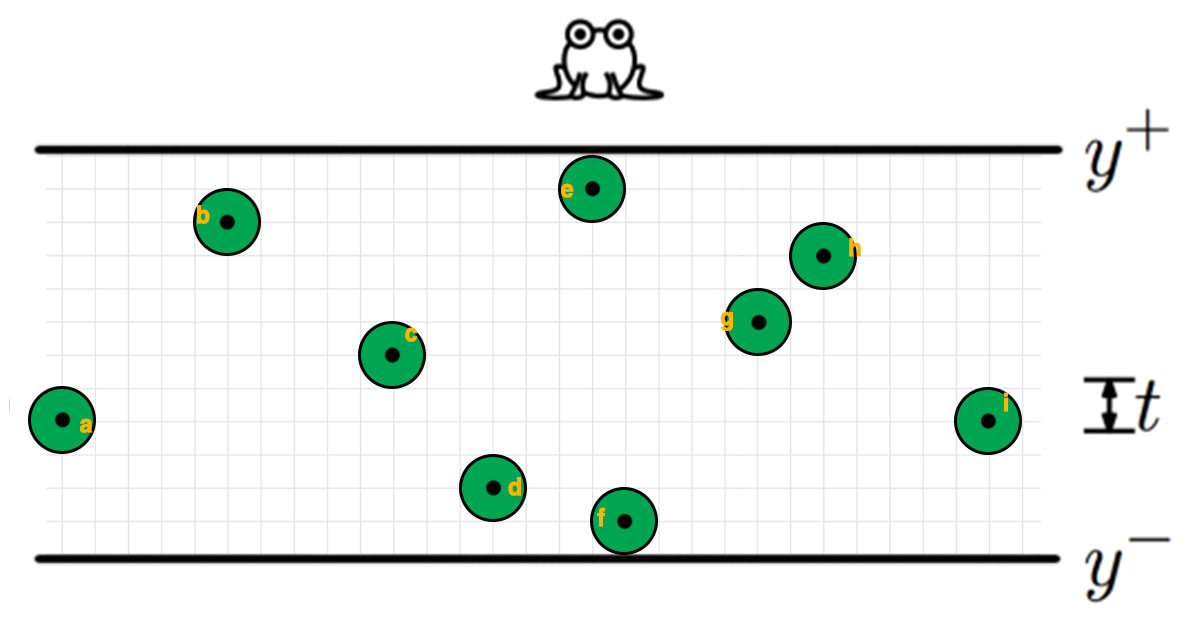
\includegraphics[scale=0.3]{img/problem2-T1.png}
	\caption{$T=1$} \label{fig:1b}
\end{figure}

\newpage
\noindent Here T=1.4, if we compute the plane Sweep we will know that $e$ intersects $y^+$, $f$ interects $y^-$ and $h$ intesercts $g$. No path exists starting from a point with a circle that intersects $y^+$ to a point with a circle that intersects $y^-$.
\begin{figure}[H]
	\centering
	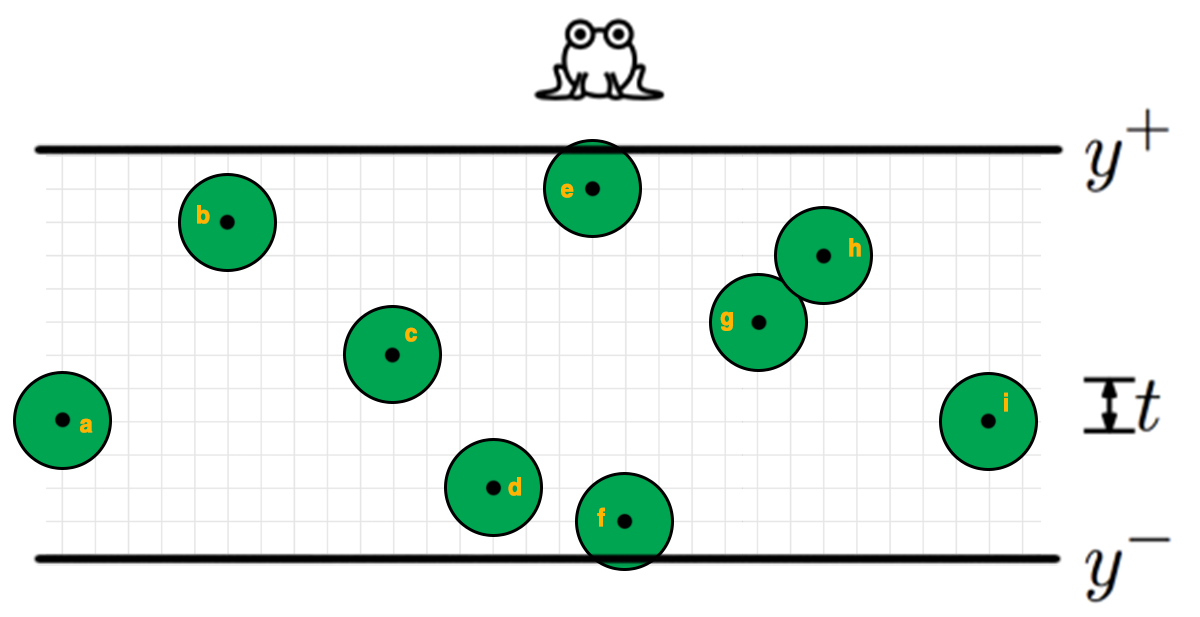
\includegraphics[scale=0.3]{img/problem2-T1_4.png}
	\caption{$T=1.4$} \label{fig:1c}
\end{figure}

\noindent Here T=2, if we compute the plane Sweep we will know that $e$ intersects $y^+$, $f$ interects $y^-$, $h$ intesercts $g$ and $d$ intesercts $f$. No path exists starting from a point with a circle that intersects $y^+$ to a point with a circle that intersects $y^-$.
\begin{figure}[H]
	\centering
	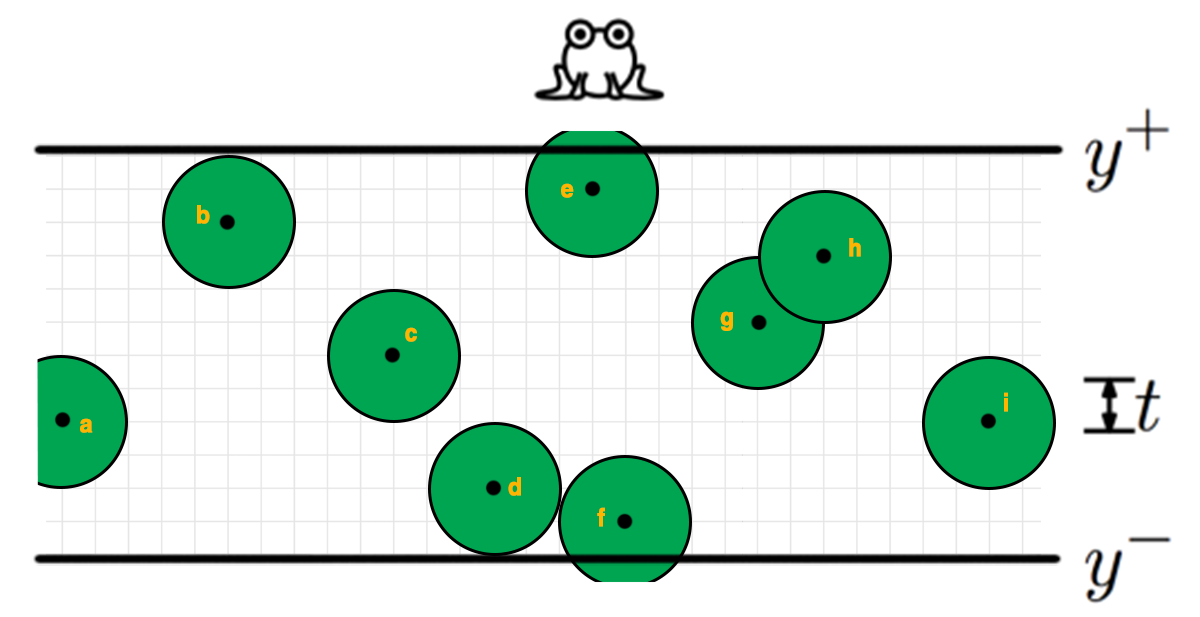
\includegraphics[scale=0.3]{img/problem2-T2.png}
	\caption{$T=2$} \label{fig:1d}
\end{figure}

\newpage
\noindent Here T=2.3, if we compute the plane Sweep we will know that $e$ intersects $y^+$, $f$ interects $y^-$, $h$ intesercts $g$, $d$ intesercts $f$ and $b$ intersects $y^+$ . No path exists starting from a point with a circle that intersects $y^+$ to a point with a circle that intersects $y^-$.
	\begin{figure}[H]
	\centering
	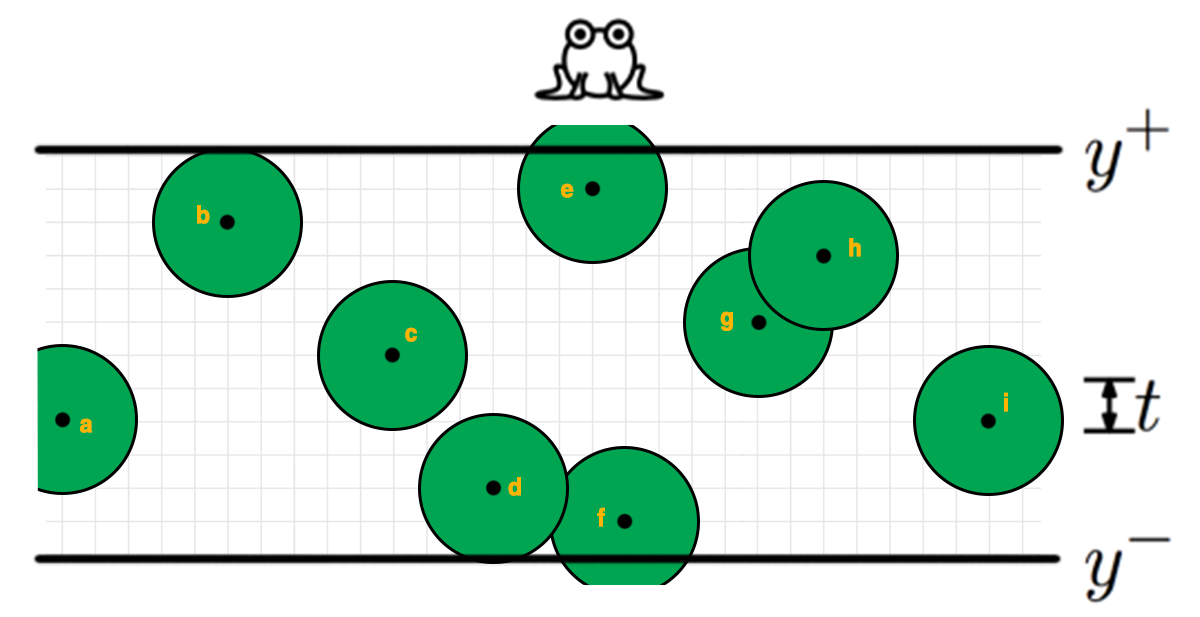
\includegraphics[scale=0.3]{img/problem2-T2_3.png}
	\caption{$T=2.3$} \label{fig:1e}
\end{figure}

\noindent Here T=3, if we compute the plane Sweep we will know that $e$ intersects $y^+$, $f$ interects $y^-$, $h$ intesercts $g$, $d$ intesercts $f$, $b$ intersects $y^+$ and $c$ intersects $d$. No path exists starting from a point with a circle that intersects $y^+$ to a point with a circle that intersects $y^-$.
\begin{figure}[H]
	\centering
	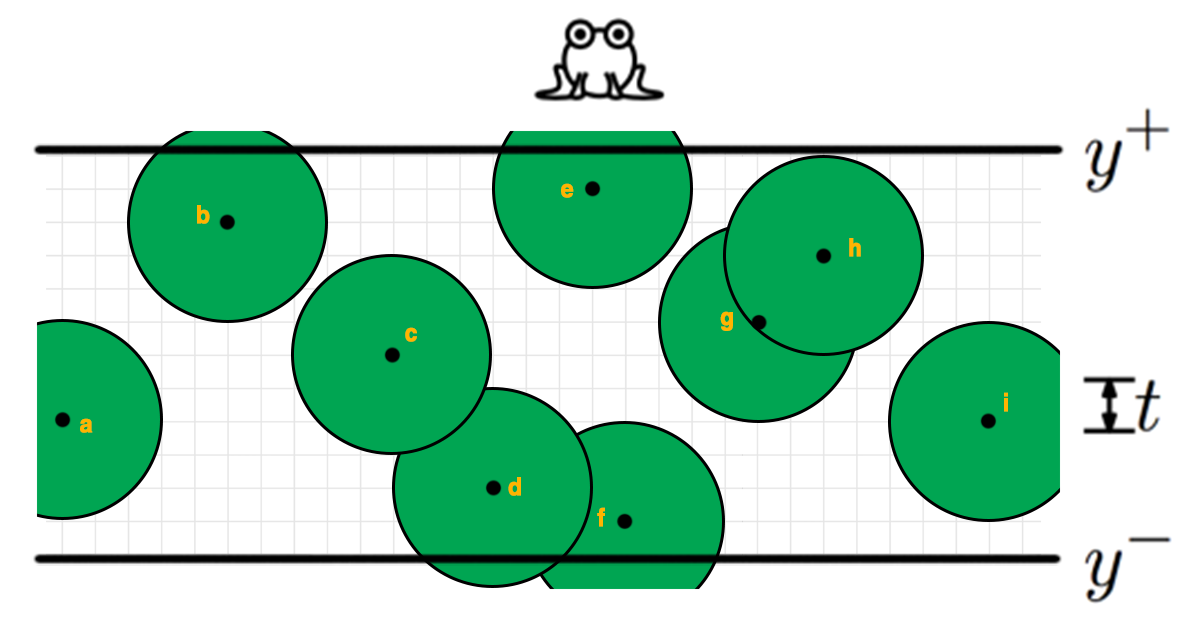
\includegraphics[scale=0.3]{img/problem2-T3.png}
	\caption{$T=3$} \label{fig:1f}
\end{figure}

\noindent Here T=3.2, if we compute the plane Sweep we will know that $e$ intersects $y^+$, $f$ interects $y^-$, $h$ intesercts $g$, $d$ intesercts $f$, $b$ intersects $y^+$, $c$ intersects $d$ and $b$ intersects $c$. It exists a path starting from a point with a circle that intersects $y^+$ to a point with a circle that intersects $y^-$. The sequence is $b \rightarrow c \rightarrow d$.
\begin{figure}[H]
	\centering
	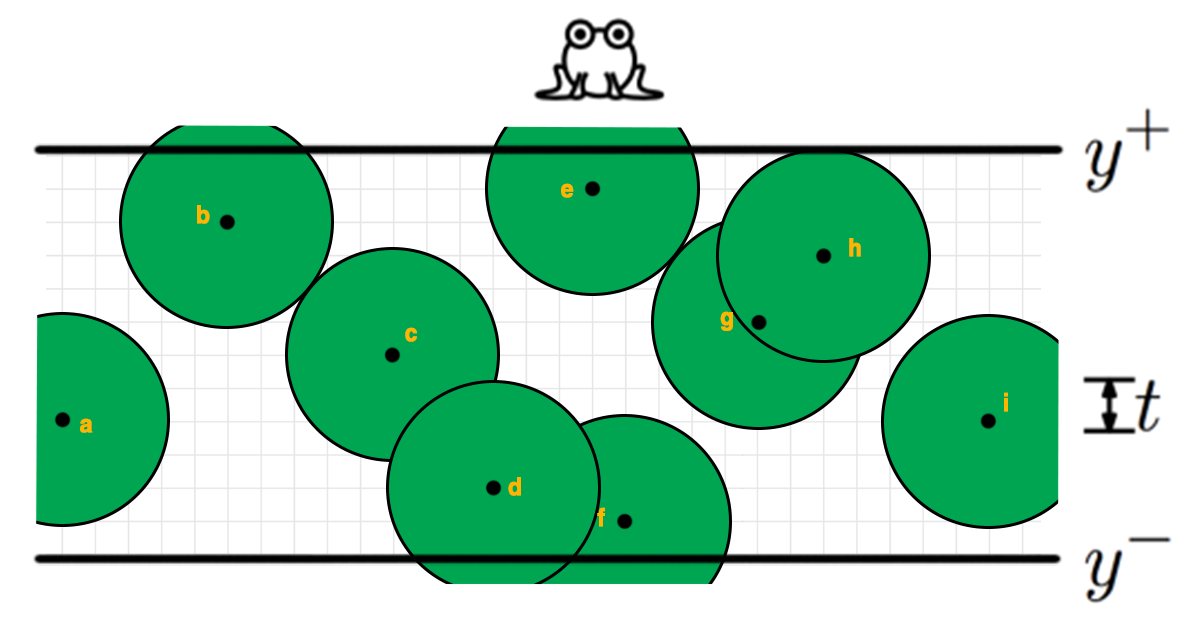
\includegraphics[scale=0.3]{img/problem2-T3_2.png}
	\caption{$T=3.2$} \label{fig:1g}
\end{figure}

\noindent \textbf{Problem 3}\\
\begin{enumerate}[label=\alph*)]
	\item Let $p,q \in P$ and let $pq$ denote an edge of the Gabriel graph of a set $P$ that we denote $G(P)$. Two sites $p$ and $q$ are connected by and edge in the Delaunay triangulation iff there is an empty circle $C_{pq}$ with diameter $pq$. By the circumcircle property, the circumcircle of any triangle in the Delaunay triangulation is "empty", that is the interior of the associated circular disk contains no sites $r \in P$. We must take into account:
	
	\begin{enumerate}[label=\roman*)]
		\item There is a point $r$ on the circle $C_{pq}$ and consequently the triangle $\Delta pqr$ to be a face of $DG(P)$, and hence the edge $pq$ become part of $DG(P)$.
		\item There is not a point $r \in P \backslash \{p,q\}$ on the circle $C_{pq}$. In this case, it must be the instance that $pq$ is an edge of the Delaunay Graph $DG(P)$.
	\end{enumerate}
	\noindent It follows that $G(P) \subseteq DG(P)$. \\
	
	\item Since our statement (ST) is an iff we can prove it from two directions:
	\begin{enumerate}[label=\roman*)]
		\item $pq$ is a Gabriel edge $\rightarrow pq$ intersects its dual Voronoi edge
		\item $pq$ intersects its dual Voronoi edge $\rightarrow pq$ is a Gabriel edge
	\end{enumerate}
			
	For (i) and (ii) we will proof by contradiction. Starting from (i) our purpose is proof that if our hypothesis ($pq$ is a Gabriel edge) it is true and the negation of our thesis $\neg (pq$ intersects its dual Voronoi edge) it is true, then this leads necessarily to a contradiction with our hypothesis, hence we can conclude that our statement (i) must be true.
	
	Therefore, if we suppose that $pq$ doesn't intersect its dual Voronoi edge then there must be a vertex $s \in P$ that belongs at the circle $C_{pq}$ centering at $m$. With the condition that if s is below $pq$ it must lie inside $C_{pq}$ centering at $o$ and this represents a contradiction of the Gabriel graph definition. Contrarily, if $s$ it is above $pq$ then it will lie inside the circle $C_{pqr}$, and therefore a contraddiction of the circumcircle property of the Delaunay triangulation. It follows that our assumption is incorrect and $pq$ must intersect its dual Voronoi edge.
	
	\begin{figure}[H]
		\centering
		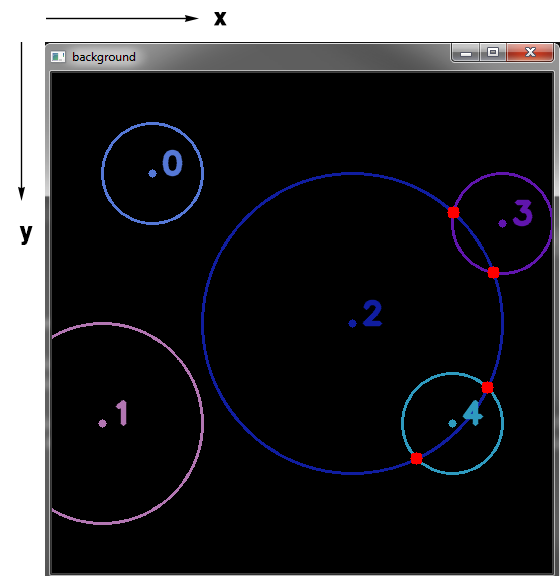
\includegraphics[scale=0.4]{img/1.png}
		\caption{proof for (i)} \label{fig:1a}
	\end{figure}
	
	On the other hand in (ii), if we negate that $pq$ represents a Gabriel edge then it exists a point $s \in C_{pq}$ centering at $o$, but it follows that $|os| < |po| = |oq|$ and for this reason $pq$ does not intersect its dual Voronoi edge. It follows that our assumption is incorrect and $pq$ is a Gabriel edge.
	
	\begin{figure}[H]
		\centering
		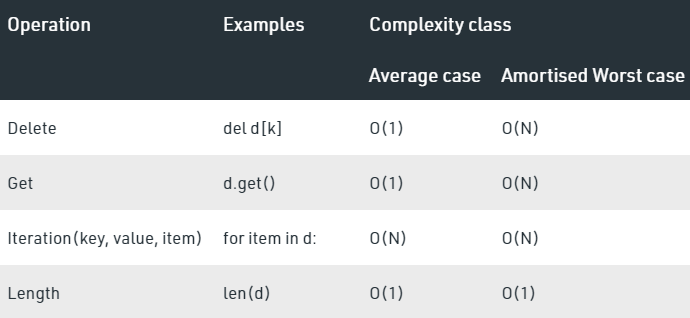
\includegraphics[scale=0.4]{img/2.png}
		\caption{proof for (ii)} \label{fig:1a}
	\end{figure}
	

	\item An algorithm to compute The Gabriel graph $G(P)$ can be:
	\begin{enumerate}[label=\roman*)]
		\item (1) Starting from the Delaunay graph of the point set $P$, hence $DG(P)$.
		\item (2) For each edge $pq \in DG(P)$, we build a circle $C_{pq}$ and if any site of $P$ lies in $C_{pq}$, we delete the edge $pq$.
	\end{enumerate}
	
	\noindent We can compute $DG(P)$ in $O(n log n)$ expected running time with a randomized incremental construction. Besides, for the in circle test, for each edge $pq \in DG(P)$, we only need to look at the neighbours of $p$ and $q$. This implies that a single vertex $r$ participates in $deg(r)$ circle violation tests. The total number of circle violation tests is $O(n)$ because $DG(P)$ is a planar graph. It follows that in general the whole algorithm requires $O(n log n) + O(n) = O(n log n)$ time.
\end{enumerate}

\end{document}